% Mumford-style picture of Spec Z[x], with the curve of x^2+1. Generated by a short script.
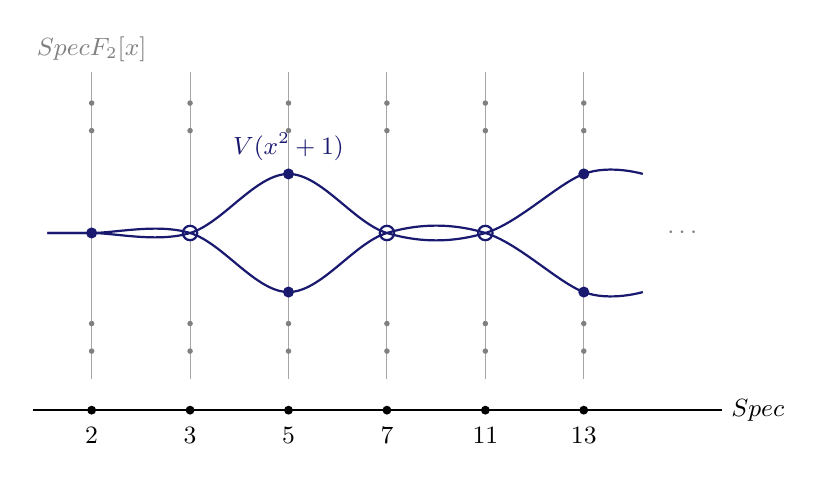
\begin{tikzpicture}[font=\small,x=1.25cm,y=1cm]
\draw[thick] (0.4,0) -- (7.4,0); \node[right] at (7.4,0) {$\operatorname{Spec}\Z$};
\draw[gray!70] (1,0.4) -- (1,4.3); \fill (1,0) circle (1.6pt); \node[below] at (1,-0.1) {$2$};
\fill[gray] (1,0.75) circle (1pt);
\fill[gray] (1,1.1) circle (1pt);
\fill[gray] (1,3.55) circle (1pt);
\fill[gray] (1,3.9) circle (1pt);
\fill[MidnightBlue] (1,2.25) circle (2pt);
\draw[gray!70] (2,0.4) -- (2,4.3); \fill (2,0) circle (1.6pt); \node[below] at (2,-0.1) {$3$};
\fill[gray] (2,0.75) circle (1pt);
\fill[gray] (2,1.1) circle (1pt);
\fill[gray] (2,3.55) circle (1pt);
\fill[gray] (2,3.9) circle (1pt);
\draw[MidnightBlue,thick,fill=white] (2,2.25) circle (2.6pt);
\draw[gray!70] (3,0.4) -- (3,4.3); \fill (3,0) circle (1.6pt); \node[below] at (3,-0.1) {$5$};
\fill[gray] (3,0.75) circle (1pt);
\fill[gray] (3,1.1) circle (1pt);
\fill[gray] (3,3.55) circle (1pt);
\fill[gray] (3,3.9) circle (1pt);
\fill[MidnightBlue] (3,3.0) circle (2pt); \fill[MidnightBlue] (3,1.5) circle (2pt);
\draw[gray!70] (4,0.4) -- (4,4.3); \fill (4,0) circle (1.6pt); \node[below] at (4,-0.1) {$7$};
\fill[gray] (4,0.75) circle (1pt);
\fill[gray] (4,1.1) circle (1pt);
\fill[gray] (4,3.55) circle (1pt);
\fill[gray] (4,3.9) circle (1pt);
\draw[MidnightBlue,thick,fill=white] (4,2.25) circle (2.6pt);
\draw[gray!70] (5,0.4) -- (5,4.3); \fill (5,0) circle (1.6pt); \node[below] at (5,-0.1) {$11$};
\fill[gray] (5,0.75) circle (1pt);
\fill[gray] (5,1.1) circle (1pt);
\fill[gray] (5,3.55) circle (1pt);
\fill[gray] (5,3.9) circle (1pt);
\draw[MidnightBlue,thick,fill=white] (5,2.25) circle (2.6pt);
\draw[gray!70] (6,0.4) -- (6,4.3); \fill (6,0) circle (1.6pt); \node[below] at (6,-0.1) {$13$};
\fill[gray] (6,0.75) circle (1pt);
\fill[gray] (6,1.1) circle (1pt);
\fill[gray] (6,3.55) circle (1pt);
\fill[gray] (6,3.9) circle (1pt);
\fill[MidnightBlue] (6,3.0) circle (2pt); \fill[MidnightBlue] (6,1.5) circle (2pt);
\node[gray] at (7.0,2.25) {$\cdots$};
\draw[MidnightBlue,thick] plot[smooth,tension=0.6] coordinates {(0.55,2.25) (1,2.25) (2,2.25) (3,3.0) (4,2.25) (5,2.25) (6,3.0) (6.6,3.0)};
\draw[MidnightBlue,thick] plot[smooth,tension=0.6] coordinates {(0.55,2.25) (1,2.25) (2,2.25) (3,1.5) (4,2.25) (5,2.25) (6,1.5) (6.6,1.5)};
\node[MidnightBlue,above] at (3.0,3.05) {$V(x^2+1)$};
\node[gray,above] at (1,4.3) {$\operatorname{Spec}\mathbb F_2[x]$};
\end{tikzpicture}
